% Evidence-checked revision, 12 September 2026. Original report/main.tex preserved.
% Build from this directory: powershell -File build.ps1
\documentclass[journal]{IEEEtran}
\usepackage[utf8]{inputenc}
\usepackage[T1]{fontenc}
\usepackage{graphicx,amsmath,amssymb,booktabs,tabularx,array,listings,xcolor}
\usepackage{tikz,pgfplots}
\usetikzlibrary{arrows.meta,positioning}
\pgfplotsset{compat=1.18}
\usepackage[hidelinks]{hyperref}
\hypersetup{pdftitle={Natural Language Task Planning for Autonomous Ground Robot Navigation via Large Language Models},pdfauthor={William Kojumian}}
\definecolor{navblue}{HTML}{174D79}
\definecolor{navorange}{HTML}{B76117}
\newcommand{\field}[1]{\texttt{#1}}
\lstset{basicstyle=\ttfamily\scriptsize,breaklines=true,columns=fullflexible,frame=single,showstringspaces=false,aboveskip=6pt,belowskip=6pt}
\newcolumntype{Y}{>{\raggedright\arraybackslash}X}
\begin{document}
\title{Natural Language Task Planning for Autonomous Ground Robot Navigation via Large Language Models}
\author{William~Kojumian\thanks{MSc Robotics, Middlesex University Dubai. Module PDE4445 Robotics Dissertation Project, 2026. Supervisor: Judhi Prasetyo.}}
\markboth{PDE4445 Robotics Dissertation Project, September 2026}{Kojumian: Natural Language Task Planning for Robot Navigation}
\maketitle

\begin{abstract}
Large language models can translate operator instructions into robot plans, but a valid output format does not establish correct task behaviour. This study evaluates typed navigation commands using a single-call gpt-4o-mini planner, a named-location JSON contract, and a ROS2 Nav2 executor for a simulated TurtleBot3 warehouse robot. A researcher-designed dataset contains 100 commands in five categories: direct, spatial, multi-step, conditional, and ambiguous. Three generation trials per command are assessed structurally; semantic assessment combines automatic matching with 27 single-rater judgements. With the revised prompt, automatic semantic success is 96.7\%, 95.0\%, and 95.0\% for the first three categories. Item-level strict scores are 55.0\% for conditional commands and 85.0\% for ambiguous commands. This descriptive reversal is consistent with unequal representational support: the contract permits clarification but cannot encode an alternative destination after failure. A targeted schema-and-prompt extension improves conditional schema adherence from 55/60 to 60/60 and passes a narrow branch-encoding check in 7/9 selected trials. These structural results support a representation bottleneck, without establishing a general causal law or improved navigation success. Three additional saved-plan replays reached all nine requested goals; semantic grading of the extension remains outstanding.
\end{abstract}
\begin{IEEEkeywords}
Large language models, robot task planning, natural language navigation, JSON schema, ROS2, Nav2, evaluation.
\end{IEEEkeywords}

\section{Introduction}
\IEEEPARstart{W}{arehouse} navigation combines repeated routes, named work areas, and changing requests~\cite{pallottino2026warehouse}. A graphical map is effective for choosing one destination. Typed language may help specify ordered patrols, responses to inaccessible areas, or requests needing clarification. This potential advantage motivates the interface; usability is not measured here.

The research question is: \emph{how reliably does translation from English to a navigation plan preserve task intent across different linguistic demands?} One successful route does not measure translator reliability, while a high plan score does not establish successful robot execution.

The prototype separates task specification from motion generation. A large language model (LLM) chooses named destinations and simple actions. An executor resolves names to map coordinates and delegates movement to Nav2. This restricted interface makes translation errors inspectable separately from physical behaviour.

Evaluation uses 100 commands divided equally among direct, spatial, multi-step, conditional, and ambiguous categories, labelled L1--L5. These are intended linguistic demands, not a validated difficulty scale. Strict scores fall at L4 and recover at L5. Explaining this pattern requires examining both the output representation and scoring rules.

The original contract permits clarification but cannot specify ``if A cannot be reached, navigate to B instead.'' Its failure options name behaviours such as retrying or skipping, not alternative destinations. Observed outputs place conditions in explanatory text while executable steps visit both destinations unconditionally.

The contribution is a reproducible command set and scoring pipeline, an analysis separating validity from task correctness, and a targeted fallback extension. This bounded case study motivates auditing the plan representation before attributing planning failures to model capacity; it does not introduce a general planning algorithm.

The scope is typed language, navigation and waiting, one known warehouse map, and simulation. ``Inspect'' and ``check'' are interpreted as navigation requests, not as implemented perception or inspection capabilities. There is no voice input, manipulation, hardware validation, or demonstrated industrial deployment readiness.

\section{Related Work}
\subsection{Language models and executable robot tasks}
SayCan grounds language-based skill selection in affordance estimates~\cite{ahn2022saycan}. Inner Monologue incorporates environment feedback into continued planning~\cite{huang2022inner}. Both already distinguish linguistic plausibility from successful embodied action; the present contribution concerns a particular navigation contract rather than discovering that plausible plans can fail.

Code as Policies generates programs with robot API calls and control structures~\cite{liang2022code}. ProgPrompt uses available actions, objects, and example programs to condition generation~\cite{singh2022progprompt}. Such representations can express branching absent from a flat waypoint contract. Here, a smaller output vocabulary trades expressiveness for inspectability; these alternatives are not experimentally compared.

Vemprala \emph{et al.} examine prompts, function libraries, and dialogue across robotics tasks~\cite{vemprala2023chatgpt}. ReAct interleaves reasoning and environment interaction~\cite{yao2023react}. Here, omitting feedback and corrective calls keeps the initial plan as the observable unit, but removes opportunities for subsequent repair.

\subsection{Language-guided navigation and the execution layer}
LM-Nav combines pretrained language, vision, and action models for navigation using language descriptions of landmarks~\cite{shah2022lmnav}. NavGPT uses textual descriptions of visual observations, navigation history, and available directions to select actions sequentially~\cite{zhou2023navgpt}. These settings include perceptual grounding or ongoing navigation context. Here, grounding is deliberately simpler: all 20 location names, descriptions, and coordinates are supplied in a known semantic map. The results therefore concern translation within a closed environment vocabulary, not landmark discovery in an unfamiliar scene.

Nav2 supplies the lower-level robotics infrastructure. The Marathon 2 describes a ROS2 navigation system with behaviour-tree orchestration~\cite{macenski2020marathon}; the later ROS2 navigation survey situates planning, control, and recovery components within that architecture~\cite{macenski2023survey}. The executor developed here operates above Nav2 and sends pose goals. It does not replace the path planner or controller. Behaviour trees can express conditional control flow, so the missing fallback is a limitation of this project's task contract rather than an inherent limitation of Nav2.

SLAM Toolbox provides mapping and localisation functionality~\cite{macenski2021slam}, but the reported simulation uses a generated occupancy map and ground-truth odometry. This isolates translation from localisation error while limiting evidence about real-world operation.

\subsection{Structured output and the research distinction}
Chain-of-thought prompting investigates explicit intermediate reasoning~\cite{wei2022chain}. The present prompts instead request a structured plan with brief explanatory fields; those fields are not executable and do not provide direct access to the model's internal reasoning. A plausible explanation accompanying an incorrect plan is evidence about the output, not proof of intact comprehension.

Tam \emph{et al.} study the effect of output-format restrictions on model performance~\cite{tam2024format}. JSONSchemaBench evaluates constrained decoding in terms of efficiency, schema coverage, and output quality~\cite{geng2025jsonschemabench}. These establish relevant distinctions between format compliance and useful content. The implementation here uses JSON-object mode plus validation after generation, not decoding constrained by the complete JSON Schema. Its schema errors are consequently observable rather than ruled out during generation.

Hallucination research provides broader context for outputs unsupported by their grounding information~\cite{ji2023hallucination}. Restricting navigation to known names addresses one narrow problem: arbitrary generated coordinates cannot become accepted coordinate fields in a conforming plan. Incorrect existing destinations, invented names, or unsupported claims in comments remain possible. Named targets are therefore an interface restriction, not a general guarantee against hallucination or unsafe action.

Table~\ref{tab:related} positions the combination of contract validation, category-based testing, and a targeted fallback intervention.

\begin{table}[t]
\caption{Relationship to selected prior work}
\label{tab:related}\centering\small
\begin{tabularx}{\columnwidth}{@{}>{\raggedright\arraybackslash}p{0.27\columnwidth}YY@{}}
\toprule
Approach & Established focus & Distinction here\\\midrule
SayCan; Inner Monologue & Affordances and feedback & Fixed map; one translation call\\
Code as Policies; ProgPrompt & Programs and situated actions & Restricted waypoint contract\\
LM-Nav; NavGPT & Language with navigation observations & Supplied named locations\\
Tam; JSONSchemaBench & Format constraints and output quality & Executable fallback semantics\\
\bottomrule
\end{tabularx}
\end{table}

\section{System Design and Implementation}
\subsection{Two paths through the prototype}
The system has a shared translation component and separate evaluation and execution paths (Fig.~\ref{fig:architecture}). The operator's typed command is sent as a user message. The system message combines the robot's role and capability limits, the semantic map, the output contract, interpretation policies, and worked examples. The planner requests gpt-4o-mini at temperature zero with \field{response\_format=json\_object}. There is one application-level generation call per command, with no agent loop or corrective re-prompting.

The evaluation runner parses the response, checks it against the selected JSON Schema, validates navigation targets against the map, and records semantic and contingency scores where applicable. The demo bridge instead writes parsed JSON to a file. The ROS2 executor reads that file or standard input, resolves destination names, and sends goals to Nav2. The current bridge does \emph{not} invoke the full evaluation validator before execution. The report therefore distinguishes the evaluated validation pipeline from the demo's more limited checks; a universal pre-execution validation gate is not claimed.

\begin{figure}[t]
\centering
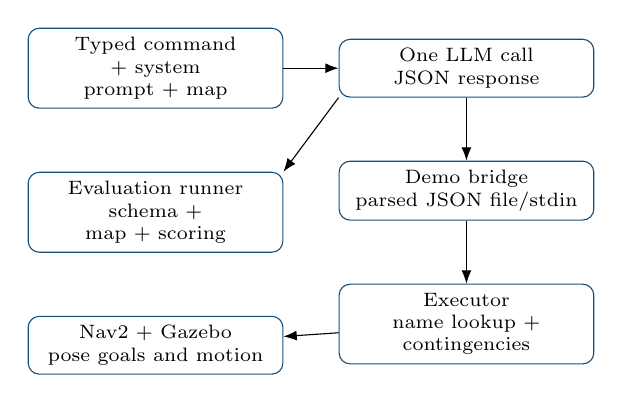
\begin{tikzpicture}[font=\scriptsize,box/.style={draw=navblue,rounded corners,align=center,minimum height=7mm,text width=30mm},>=Latex]
\node[box] (input) {Typed command\\+ system prompt + map};
\node[box,right=7mm of input] (llm) {One LLM call\\JSON response};
\node[box,below=8mm of input] (eval) {Evaluation runner\\schema + map + scoring};
\node[box,below=8mm of llm] (file) {Demo bridge\\parsed JSON file/stdin};
\node[box,below=8mm of file] (exec) {Executor\\name lookup + contingencies};
\node[box,below=8mm of eval] (nav) {Nav2 + Gazebo\\pose goals and motion};
\draw[->] (input)--(llm);
\draw[->] (llm)--(file);
\draw[->] (llm.south west)--(eval.north east);
\draw[->] (file)--(exec);
\draw[->] (exec)--(nav);
\end{tikzpicture}
\caption{Implemented evaluation and demo paths. Full schema and map validation belongs to the evaluation runner; the demo bridge does not currently enforce that same gate.}
\label{fig:architecture}
\end{figure}

\subsection{Map and plan contract}
The semantic map describes a $20\times20$\,m warehouse with three aisles and 20 named locations. North is positive $y$ and east is positive $x$. Each name maps to fixed coordinates and a textual description. The model can use those coordinates when interpreting ``nearest'' or ``midway,'' but its navigation output is a name. The executor alone converts that name into a pose. This makes the map the authority for destination coordinates.

At plan level, \field{understood} indicates whether the model accepts the request. The prompt asks for an empty plan and a useful \field{clarification\_question} when it does not. At step level, \field{navigate} identifies a target, while \field{wait} supplies \field{duration\_s}. The \field{reason} and \field{notes} fields explain choices but have no control-flow effect. In particular, a condition written in either field does not make a later navigation step conditional.

Table~\ref{tab:contingency} describes the implemented v2 failure actions. These run after a navigation attempt reports failure. A failed attempt is used as an approximation to ``blocked''; there is no separate semantic detector for an occupied dock, noise source, or blocked-aisle count. Nav2 may already have attempted its own recoveries before returning failure.

\begin{table}[t]
\caption{Executor behaviour after a navigation failure (v2)}
\label{tab:contingency}\centering\small
\begin{tabularx}{\columnwidth}{@{}p{0.38\columnwidth}Y@{}}
\toprule
\field{on\_blocked} & Executed response\\\midrule
\field{abort} & Stop the remaining plan.\\
\field{skip} & Mark the step skipped; continue.\\
\field{wait\_retry} & Wait, then retry the same target once; default wait is 5\,s.\\
\field{reroute\_perimeter} & Visit a route on the perimeter and retry access to the original destination.\\
\field{null} & Record failure; continue to later steps.\\
\bottomrule
\end{tabularx}
\end{table}

The JSON Schema checks declared types, enumerations, and disallowed extra properties, but some prompt requirements exist only as descriptions. For example, the v2 schema does not formally enforce every relationship between acceptance, clarification, action, target, and wait duration. A schema pass therefore establishes compliance with the implemented validator, not every intended contract rule. Similarly, map membership does not establish traversability, clearance, or preservation of the operator's intent.

\subsection{Prompt architecture and revisions}
The v2 prompt contains 13 interpretation policies and six worked examples after the contract and map. Policies define traversal versus endpoint navigation, sequence preservation, wall sweeps, perimeter direction, geometric inference, waiting, contingencies, ambiguity, capability limits, and home/base aliases. This is task-specific prompting with examples, rather than model training or fine-tuning.

Seven documented changes distinguish v2 from v1: separate endpoint requests from aisle traversals; infer from map descriptions before clarifying; define clockwise and counter-clockwise order explicitly; expand wall sweeps to corner--midpoint--corner; choose a named point for geometric descriptions; translate ``wait at X'' into navigation followed by waiting; and explicitly request \field{wait\_retry} for retry instructions. The revisions target observed error categories. Because they followed inspection of evaluation failures and reuse the same dataset, their measured improvement is a development-set result, not held-out generalisation.

There is direct overlap between prompt examples and test commands: v2 includes the exact text of L1-01, L2-03, and L4-09. General policies can still be useful, but example overlap prevents describing the comparison as free from test exposure. The baseline records are evaluated under the archived contract that includes \field{wait\_retry}; the comparison does not establish an isolated historical schema change for v1 versus v2.

\subsection{Simulation and motion execution}
The robot is a TurtleBot3 Waffle in Gazebo Classic 11 under ROS2 Humble in WSL2. A script generates the occupancy grid and warehouse geometry from common dimensions. Grid resolution is 0.05\,m, giving a $400\times400$ map. Aisle centre lines lie at $x=6$, 9, and 12\,m. All 20 named locations were checked against the stored grid and occupy free cells; this check does not by itself certify footprint clearance or feasible routes.

Localisation for the demonstrated configuration uses simulator ground-truth odometry, a map server, and a static identity transform from \field{map} to \field{odom}. SLAM Toolbox is not running in this path. The launch file also offers AMCL, but that alternative is not the basis of the reported result. Ground truth reduces localisation uncertainty, allowing the experiment to concentrate on plan translation and integration.

Nav2 uses NavFn for global planning and Regulated Pure Pursuit for path following in the stored configuration. Desired linear velocity is 0.26\,m/s; configured goal tolerances are 0.25\,m in position and 0.25\,rad in yaw. The executor constructs map-frame pose goals and calls \field{BasicNavigator.goToPose}. Goal orientation is derived from the previous recorded position towards the next target; the language contract does not specify approach direction or final orientation.

The ROS-free \field{plan\_runner.py} implements sequencing, waiting, and failure handling. Seven existing mock-based tests pass, covering simple navigation, clarification without execution, abort, skip, retry, perimeter rerouting, and waiting. These verify selected control paths, not complete JSON validation or physical navigation. The ROS adapter reads a file or stdin and logs outcomes; it does not subscribe to a plan topic or publish a dedicated plan-status topic.

\subsection{Engineering observations and demonstration}
Development notes record communication problems with Fast DDS under WSL2 and a working configuration using Cyclone DDS restricted to loopback. They also record action-handshake timeouts in an uncomposed Nav2 launch and successful operation after composition. The checked-in launch hosts the navigation stack in a component container. These observations justify the chosen configuration, but no controlled middleware benchmark establishes a unique root cause or general performance improvement.

The archived demonstration requests: ``Sweep aisle 1, check the packing station and the loading dock, then return to base.'' Its five goals are \field{aisle\_1\_south}, \field{aisle\_1\_north}, \field{packing\_station}, \field{loading\_dock}, and \field{charging\_dock}. The saved replay reports 5/5 goals reached, with a corresponding trajectory. This is the route supported by the stored artifact; it differs from the illustrative two-aisle patrol used elsewhere in development notes.

\begin{figure}[t]
\centering
\begin{tikzpicture}
\begin{axis}[width=.88\columnwidth,height=.88\columnwidth,axis equal image,
xmin=0,xmax=20,ymin=0,ymax=20,xtick={0,5,10,15,20},ytick={0,5,10,15,20},
xlabel={East (m)},ylabel={North (m)},tick label style={font=\scriptsize},label style={font=\scriptsize},
grid=major,grid style={gray!15},axis on top]
\fill[gray!45] (axis cs:4.25,4) rectangle (axis cs:4.75,13);
\fill[gray!45] (axis cs:7.25,4) rectangle (axis cs:7.75,13);
\fill[gray!45] (axis cs:10.25,4) rectangle (axis cs:10.75,13);
\fill[gray!45] (axis cs:13.25,4) rectangle (axis cs:13.75,13);
\addplot[navorange,thick,no marks] table[x=x,y=y]{trajectory.dat};
\addplot[only marks,mark=*,navblue,mark size=2pt] coordinates {(6,4)(6,16)(15,10)(18,2)(1,1)};
\node[font=\scriptsize,anchor=north west] at (axis cs:6,4) {1};
\node[font=\scriptsize,anchor=south] at (axis cs:6,16) {2};
\node[font=\scriptsize,anchor=south east] at (axis cs:15,10) {3};
\node[font=\scriptsize,anchor=south west] at (axis cs:18,2) {4};
\node[font=\scriptsize,anchor=south west] at (axis cs:1,1) {5};
\end{axis}
\end{tikzpicture}

\caption{Warehouse shelf geometry and archived demo trajectory. The numbered goals are aisle 1 south (1), aisle 1 north (2), packing station (3), loading dock (4), and charging dock (5). The plotted trace is stored odometry, not a newly executed experiment.}
\label{fig:warehouse}
\end{figure}

This demonstration establishes multi-goal integration, not a mission-success probability, physical inspection, or conditional behaviour. It is separate from the plan-level evaluation.

Follow-up checks on 12 September replayed three saved v2 outputs (trial 0): L1-01 reached 1/1 goals, L2-01 reached 3/3, and L3-01 reached 5/5. Each used a fresh headless world and the unchanged executor. Recorded odometry corroborated all nine destinations within the configured 0.25\,m tolerance. An initial attempt lacked a resolved ground-plane model, followed by a startup timeout; both are retained as environment failures. The successful replays followed model-path and process-cleanup repairs. These selected single runs add execution evidence, not independent language samples or conditional-recovery validation.

\section{Evaluation Method}
\subsection{Dataset and generation protocol}
The dataset contains 20 commands per category (Table~\ref{tab:levels}). Items are authored around a fixed map and expected robot capabilities. L1--L3 use accepted destination sequences or required-visit rules; L4 includes both automatically checkable contingencies and rubric cases; L5 combines resolvable defaults, missing information, nonexistent locations, and capability limits. Thus, the categories vary in more than sentence complexity.

\begin{table}[t]
\caption{Command categories and dataset examples}
\label{tab:levels}\centering\small
\begin{tabularx}{\columnwidth}{@{}clY@{}}
\toprule
Level & Category & Example\\\midrule
L1 & Direct & Go to the loading dock.\\
L2 & Spatial & Move along the east wall from south to north.\\
L3 & Multi-step & Patrol aisles 1 and 3, then return to the charging dock.\\
L4 & Conditional & Inspect storage zone A; if unreachable, inspect zone B instead.\\
L5 & Ambiguous & Go check that thing near the door.\\
\bottomrule
\end{tabularx}
\end{table}

The main v1 and v2 runs were saved on 1 August 2026. Each contains three generation trials for all 100 commands, giving 300 records per prompt version. The v3 run, saved on 7 August, repeats only the 20 L4 commands, producing 60 records. All use the recorded model identifier gpt-4o-mini and temperature zero. These are repeated outputs for the same commands, not additional independent command samples. The record identifies the model alias rather than an immutable model snapshot, limiting exact future reproducibility.

Each record stores the command ID, trial, raw response, latency, parse status, schema and map errors, and scoring fields. No new model calls were made for this report revision. The analysis uses the archived files and grades; it does not replace missing manual judgements with inferred passes.

\subsection{Four evaluation measures}
\emph{Parse validity} asks whether the response can be decoded as JSON. \emph{Schema adherence} asks whether the parsed object passes the chosen schema. \emph{Map validity} asks whether navigation targets exist in the semantic map. \emph{Semantic correctness} asks whether the represented task matches the instruction under the dataset's matching rules or rubric. The checks are conceptually distinct but operationally sequential: schema rejection prevents later scoring in the runner.

For automatic semantic scoring, sequence items compare ordered navigation-target lists against accepted alternatives. Required-visit items check destination membership and, where specified, order, forbidden locations, or the existence of a wait action. Contingency expectations are recorded separately. These checks are reproducible but incomplete proxies for behaviour: they do not generally validate wait durations, physical route geometry, or every action relationship. A destination-list match should not be interpreted as complete executable equivalence.

The runner checks map membership only after schema success. Consequently, an unpopulated \field{map\_error} on a schema-invalid record is not evidence of map validity. Reported map-check counts include only responses that actually reached that stage. For v3, the unchanged map checker inspects ordinary navigation targets but does not validate \field{fallback\_target}; the narrow branch diagnostic checks selected expected fallback names separately.

\subsection{Manual grading and denominators}
There are 28 rubric-designated commands: 11 at L4 and 17 at L5. L4-08 fails schema validation in every v2 trial and does not enter manual semantic grading. The archived grading sheet therefore contains 27 items: 10 L4 and 17 L5. Their displayed outputs correspond to the first stored generation, apart from a punctuation-encoding difference in L5-18. Each was graded once by one researcher.

The recorded categories are pass, partial, and fail. The strict judgement reserves a pass for an acceptable represented response; partial credit records cases with some intended content but incorrect or incomplete executable behaviour. In particular, naming an alternative destination in comments or later unconditional steps can satisfy a permissive rubric description yet receive only partial credit under the stricter behavioural interpretation. This distinction must remain visible because it affects the central finding.

Development notes describe a blind, shuffled procedure with seed 4445. However, the archived v2 grading interface identifies v2 in its heading and displays items in ID order. The stored artifact therefore does not establish effective blinding or that shuffle. This report treats the labels as single-researcher judgements, without asserting independent blinded assessment or inter-rater agreement~\cite{artstein2008agreement}.

For L1--L3, strict rates use 60 generation records per level. For L4--L5, the descriptive summary combines the stable automatic item outcomes with the once-graded rubric items, giving 20 item outcomes per level. Specifically, L4 has nine automatic passes plus two manual passes, six partials, and three failures; L5 has three automatic passes plus 14 manual passes and three partials. The L4 item summary does not incorporate the later schema-invalid generations of L4-17 and L4-19 as additional manual failures.

For $N$ outcomes, $P$ passes, and $H$ partials, the reported scores are
\begin{equation}
 S_{\mathrm{strict}}=\frac{P}{N},\qquad
 S_{\mathrm{weighted}}=\frac{P+0.5H}{N}.
\end{equation}
The weighted score is partial credit, not the proportion of fully successful tasks. No pooled success rate is computed across the mixed denominators. The L4--L5 comparison additionally reports descriptive Wilson intervals and a two-sided Fisher exact test on pass versus non-pass, with the qualifications in Section~\ref{sec:threats}.

\subsection{Targeted fallback intervention}
Version v3 adds \field{goto\_fallback} and \field{fallback\_target} to the contract. The associated prompt policy explicitly instructs the model to place the alternative on the failed step and not emit it as a later unconditional navigation. The schema requires a nonempty fallback string when the new action is selected. This is one conceptual feature implemented through coordinated schema and prompt changes, not a schema-only ablation.

The structural comparison tests L4 schema adherence and a diagnostic subset of three commands: L4-12, L4-13, and L4-17. A branch passes that diagnostic when the first emitted fallback has the specified destination and that destination is not repeated in subsequent unconditional navigation targets. The check is intentionally narrower than complete semantics: it does not establish correct trigger attachment, traversal geometry, recovery after fallback failure, or executable robot behaviour. The v2 baseline is zero by construction because the field does not exist. The archived executor has no \field{goto\_fallback} implementation, so v3 is evaluated as a representation experiment only.

\section{Results and Analysis}
\subsection{Structural validity}
All 300 v2 responses parse as JSON. L1, L2, L3, and L5 each have 60/60 schema-valid responses. L4 has 55/60, giving 295/300 overall. All 295 responses reaching the ordinary-target map check pass it. Table~\ref{tab:structural} separates the checks to avoid assigning unperformed checks a success.

\begin{table}[t]
\caption{Structural checks on v2 generation records}
\label{tab:structural}\centering\small
\begin{tabular}{@{}lrrr@{}}
\toprule
Level & JSON parses & Schema passes & Map passes/checks\\\midrule
L1 & 60/60 & 60/60 & 60/60\\
L2 & 60/60 & 60/60 & 60/60\\
L3 & 60/60 & 60/60 & 60/60\\
L4 & 60/60 & 55/60 & 55/55\\
L5 & 60/60 & 60/60 & 60/60\\\midrule
Total & 300/300 & 295/300 & 295/295\\
\bottomrule
\end{tabular}
\end{table}

The five rejected L4 responses contain eight out-of-enum \field{on\_blocked} fields using three distinct values. L4-08 emits \field{wait} twice in each of its three responses (six fields). L4-17 emits \field{navigate} once and L4-19 emits \field{try\_aisle\_1\_north} once. Thus, ``three values,'' ``five responses,'' and ``eight fields'' describe different counts. The last value is particularly suggestive of an attempted alternative destination. The \field{wait} errors also show that not every violation is explained by the absence of destination fallback: a retry behaviour already exists.

\subsection{Prompt revision and repeatability}
On L1--L3, v1 obtains 54/60, 48/60, and 51/60 automatic semantic passes; v2 obtains 58/60, 57/60, and 57/60. The combined result is 153/180 (85.0\%) versus 172/180 (95.6\%), an increase of 19 passing records or 10.6 percentage points. Table~\ref{tab:prompt} also gives the three-trial mean in passes per 20 commands.

\begin{table}[t]
\caption{Automatic semantic results for the prompt comparison}
\label{tab:prompt}\centering\small
\begin{tabular}{@{}lrrrr@{}}
\toprule
& \multicolumn{2}{c}{Passing records / 60} & \multicolumn{2}{c}{Mean passes / 20}\\
Level & v1 & v2 & v1 & v2\\\midrule
L1 & 54 & 58 & 18.0 & 19.3\\
L2 & 48 & 57 & 16.0 & 19.0\\
L3 & 51 & 57 & 17.0 & 19.0\\
\bottomrule
\end{tabular}
\end{table}

Seven commands improve on L1--L3 and none regress. The often-quoted total of eight improved commands includes L5-13, outside that three-level comparison. Because revisions were developed after inspecting failures and some examples overlap with test items, these gains demonstrate improvement on this command set rather than unbiased performance on unseen requests.

Across all five categories, the recorded scoring outcomes remain identical over trials for 99/100 commands under v1 and 97/100 under v2. The three varying v2 cases are L1-18, L4-17, and L4-19. This is score repeatability, not output determinism: comparing full parsed JSON objects, including comments, yields identical objects for only 43/100 v1 commands and 50/100 v2 commands. Stable scores can conceal different explanations or plans that share the same score. Temperature zero therefore does not justify treating the output as invariant.

\subsection{Category scores and the L4--L5 contrast}
Table~\ref{tab:semantic} and Fig.~\ref{fig:reliability} show the descriptive pattern. Strict rates on L1--L3 are 96.7\%, 95.0\%, and 95.0\%. L4 has 11 passes, six partials, and three failures, giving 55.0\% strict and 70.0\% weighted. L5 has 17 passes and three partials, giving 85.0\% strict and 92.5\% weighted. L5 exceeds L4 but remains below L1--L3.

\begin{table}[t]
\caption{Semantic summary with explicit scoring units}
\label{tab:semantic}\centering\small
\begin{tabular}{@{}llrr@{}}
\toprule
Level & Scoring unit & Strict & Weighted\\\midrule
L1 & 60 records; 58 pass & 96.7\% & 96.7\%\\
L2 & 60 records; 57 pass & 95.0\% & 95.0\%\\
L3 & 60 records; 57 pass & 95.0\% & 95.0\%\\
L4 & 20 items; 11 pass & 55.0\% & 70.0\%\\
L5 & 20 items; 17 pass & 85.0\% & 92.5\%\\
\bottomrule
\end{tabular}
\end{table}

\begin{figure}[t]
\centering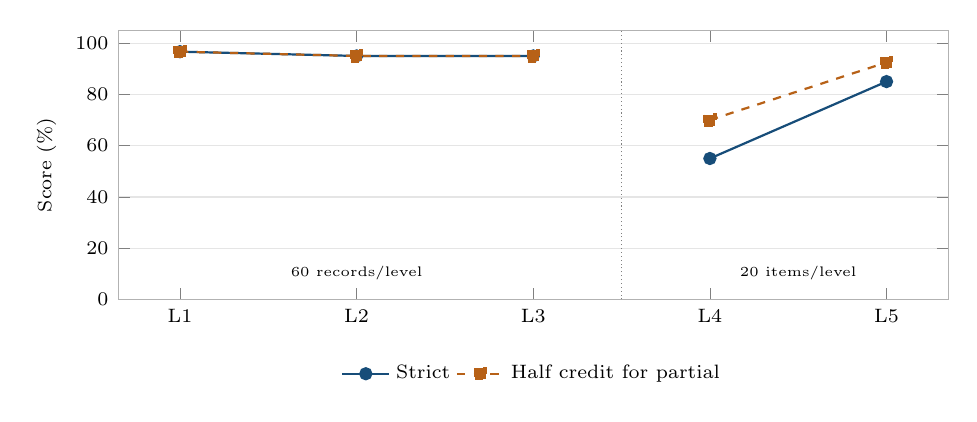
\begin{tikzpicture}
\begin{axis}[width=\columnwidth,height=5cm,ymin=0,ymax=105,xmin=.65,xmax=5.35,
xtick={1,2,3,4,5},xticklabels={L1,L2,L3,L4,L5},ytick={0,20,40,60,80,100},
ylabel={Score (\%)},tick label style={font=\scriptsize},label style={font=\scriptsize},
ymajorgrids=true,grid style={gray!20},axis line style={gray!60},
legend style={font=\scriptsize,draw=none,at={(.5,-.2)},anchor=north,legend columns=2}]
\addplot[navblue,thick,mark=*] coordinates {(1,96.6667)(2,95)(3,95)};
\addlegendentry{Strict}
\addplot[navorange,thick,dashed,mark=square*] coordinates {(1,96.6667)(2,95)(3,95)};
\addlegendentry{Half credit for partial}
\addplot[navblue,thick,mark=*,forget plot] coordinates {(4,55)(5,85)};
\addplot[navorange,thick,dashed,mark=square*,forget plot] coordinates {(4,70)(5,92.5)};
\draw[gray,densely dotted] (axis cs:3.5,0)--(axis cs:3.5,105);
\node[font=\tiny,anchor=south] at (axis cs:2,4) {60 records/level};
\node[font=\tiny,anchor=south] at (axis cs:4.5,4) {20 items/level};
\end{axis}
\end{tikzpicture}

\caption{v2 semantic scores. L1--L3 use repeated automatic records; L4--L5 combine automatic item outcomes with once-graded rubric outputs. The separation marks the change in scoring unit. Connecting segments guide the eye and do not imply a calibrated difficulty scale.}
\label{fig:reliability}
\end{figure}

The 30-percentage-point L4--L5 difference is descriptive. With 20 items per category, 95\% Wilson intervals are 34.2--74.2\% for L4 and 64.0--94.8\% for L5. A two-sided Fisher exact test on $[11,9]$ versus $[17,3]$ gives $p=0.0824$, not below 0.05. These calculations neither prove equality nor establish a population-level reversal. The authored categories and unequal success criteria further limit inference. The stronger argument concerns identifiable encoding failures and the targeted intervention.

\subsection{Clarification and missing conditional structure}
In the first v2 generation, 11/20 L5 responses defer using \field{understood=false}. L5-18, ``Go to aisle 5,'' correctly asks which of the three existing aisles is intended. That is an appropriate response for this rubric, but it completes no navigation task. Clarification is not automatically correct for every ambiguous-looking instruction: map descriptions or an accepted default can make a request resolvable. L5 success measures an acceptable response policy, including deferral, rather than the rate of completed robot missions.

Alternative-destination conditionals expose a different requirement. L4-12 requests inspection of zone A, with zone B only if A is unreachable. The first v2 output places A and B in separate ordinary navigation steps. Its second step contains the reason ``Navigate to storage zone B if storage zone A is unreachable.'' The executor does not interpret this sentence. With successful navigation to A, it still proceeds to B, contradicting the requested condition.

The following projection retains the relevant executable fields of that saved response; explanatory fields are omitted for compactness.
\begin{lstlisting}
"plan": [
  {"action": "navigate",
   "target": "storage_zone_a",
   "on_blocked": "reroute_perimeter"},
  {"action": "navigate",
   "target": "storage_zone_b",
   "on_blocked": null}
]
\end{lstlisting}

This output recognises the conditional wording in its explanation but does not preserve it in executable structure. That observation is consistent with a representation bottleneck. It cannot establish that the model's comprehension is otherwise perfect, since the explanation itself is generated text and the prompt explicitly directs residual alternatives into notes. The observed behaviour may reflect both the restricted contract and the instructed workaround.

The ten manually graded L4 cases help localise the limitation (Table~\ref{tab:taxonomy}). Retry requests pass where a corresponding action exists. Six partials involve alternative or contingent follow-on behaviour, but they are not six instances of a simple single-target fallback. They include multi-waypoint tasks, aggregate conditions, and recovery after fallback failure. This distinction is necessary to interpret v3's scope.

\begin{table}[t]
\caption{Descriptive taxonomy of manually graded L4 items}
\label{tab:taxonomy}\centering\small
\begin{tabularx}{\columnwidth}{@{}Yp{.29\columnwidth}l@{}}
\toprule
Requested structure & IDs (L4-) & Grades\\\midrule
Retry the same destination & 09, 16 & 2 pass\\
Alternative/follow-on task & 02, 12, 13, 17, 19 & 5 partial\\
Aggregate condition & 10, 15 & partial, fail\\
Approach geometry & 20 & fail\\
\bottomrule
\end{tabularx}
\end{table}

\subsection{What v3 repairs, and what it does not}
For the 60 L4 records, v3 raises schema adherence from 55/60 to 60/60. The eight out-of-enum field occurrences disappear. On the selected branch diagnostic, L4-12 and L4-13 pass in all three trials. L4-17 passes in one trial; in the other two it names the fallback but also visits it unconditionally. The resulting 7/9 is a structural encoding result over three selected commands, not a semantic success rate over L4.

\begin{table}[t]
\caption{L4 intervention: measured structural outcomes}
\label{tab:v3}\centering\small
\begin{tabularx}{\columnwidth}{@{}Yrr@{}}
\toprule
Measure & v2 & v3\\\midrule
Schema-valid responses & 55/60 & 60/60\\
Invalid contingency-field occurrences & 8 & 0\\
Selected branch diagnostic & 0/9 & 7/9\\
L4 semantic pass rate & 55\%$^{a}$ & Ungraded\\
\bottomrule
\multicolumn{3}{@{}l}{\scriptsize $^{a}$Item-level v2 summary; not 60 graded generations.}
\end{tabularx}
\end{table}

The baseline diagnostic is zero because the old contract cannot express the field being tested. The informative observation is therefore how often the new representation is used without flattening the branch. Since v3 also changes the prompt policy, this result supports the combined intervention; it does not isolate the independent causal effect of schema syntax.

Several residual requirements exceed a single fallback destination. L4-02 needs an alternative multi-waypoint patrol. L4-10 and L4-15 require state aggregated over blocked aisles. L4-20 requires approach geometry. L4-19 additionally asks for termination if the alternative also fails; it lies outside the three-command diagnostic and still repeats its fallback unconditionally in all three v3 outputs. Together with the two L4-17 failures, this prevents claiming that every remaining error lies outside the feature's intended scope.

The new field is neither executed nor completely validated by the current downstream stack. The executor has no handler for it, and the ordinary map validator does not inspect its target. Moreover, 33/60 v3 records remain marked manual. Schema adherence and branch placement are useful intermediate outcomes, but successful task execution requires the schema, semantic checks, and executor to share the same meaning. That integration and independent semantic grading remain unfinished.

\subsection{Response latency}
For the 300 v2 records, mean measured latency is 2.23\,s, median 2.08\,s, and the 95th percentile 3.63\,s. The percentile uses Python's exclusive quantile interpolation; an inclusive convention gives 3.56\,s on the same observations. The timer begins before client construction and ends after the response is received, before JSON parsing and validation. These values describe observed planner-call latency, including local client and network overhead, rather than pure model inference time or robot mission duration. No real-time or deployment service-level guarantee is inferred.

\section{Discussion and Threats to Validity}
\label{sec:threats}
\subsection{Interpretation and practical significance}
The representational limitation is straightforward once identified. The empirical contribution locates it in saved plans, distinguishes it from parsing and map errors, and tests an intervention with a measurable boundary. A larger model may improve selection among representable plans, but cannot make an unimplemented field executable without changing the surrounding system.

The practical implication is to check whether the vocabulary expresses the required behaviour, the validator checks it, and the executor implements it. Here, v2 has valid but unconditional alternatives, while v3 emits branches its executor cannot run. A syntactic improvement alone does not establish a robotics improvement.

\subsection{Unequal response policies and construct validity}
The L4--L5 contrast has a scoring confound. L5 often passes by appropriately declining to act, while L4 generally requires a specific conditional plan. The representation provides a deferral mechanism but lacks some conditional mechanisms, so the asymmetry is both part of the proposed explanation and a reason not to interpret the score gap as a pure language-complexity effect. A stronger evaluation would report correct execution plans, appropriate deferrals, and inappropriate deferrals separately under predefined task requirements.

L1--L5 is a researcher-designed taxonomy, not a psychometrically or linguistically validated ordinal scale. Ambiguity, sequence length, spatial grounding, and conditional control are different dimensions. Success need not decrease monotonically with those labels, even for a better planner. The defensible claim is that representational support helps explain this dataset's error distribution; the experiment does not show that linguistic complexity has no effect.

\subsection{Researcher choices, grading, and statistical limits}
One researcher designed the schema, dataset, prompts, expected plans, and manual judgements. Prompt revision used observed failures; three examples exactly match dataset items. There is no held-out test set, independent dataset designer, external baseline, or comparison across model sizes. The absolute 55\% L4 score consequently has no external reference point, and the v1--v2 gain may reflect adaptation to the development set.

Manual grading uses only one output per rubric item, while other categories use three generations. The strict interpretation is more demanding than parts of the original rubric, and the saved interface does not substantiate blinding. A second rater, a frozen rubric, and agreement measurement would improve confidence~\cite{artstein2008agreement}. Repeated generations should be analysed as clustered within commands; counting all three as independent task samples would exaggerate precision. The reported intervals and Fisher test are descriptive diagnostics on authored items, not design-based estimates for all warehouse language.

The v3 subset is selected around an anticipated feature benefit, and its zero baseline is definitional. The intervention changes prompt instructions as well as the schema and was run on a later date using a model alias. Without a schema-by-prompt ablation or immutable model snapshot, attribution remains limited. Complete v3 semantic grades are needed before claiming an improvement in task correctness.

\subsection{Robotics and deployment limits}
Navigation evidence comprises the archived demonstration and three selected replays, one run per replay after environment repair. Most outcomes remain plan judgements, not observed robot behaviour. The fixed map, ground-truth localisation, static warehouse, and simulated platform remove important sources of real-world uncertainty. No systematic experiments quantify obstacle-triggered branches, localisation drift, collisions, mission duration, or recovery success.

The implementation also lacks a common validation gate across evaluation and execution, complete cross-field schema constraints, and v3 fallback execution. ``Blocked'' is inferred from goal failure, and named-waypoint matching cannot prove an exact patrol path or physical inspection. These limitations preclude a safety guarantee or a supported claim of operational deployment maturity. They do not invalidate the saved translation results, but they constrain what those results establish about a robot.

\section{Conclusion and Future Work}
On this development dataset, typed language translates into restricted navigation plans with automatic semantic scores near 95\% for direct, spatial, and multi-step requests. Conditional commands score below ambiguous commands, but that descriptive difference is not statistically conclusive and does not isolate linguistic difficulty.

Saved failures identify representation as one limiting factor: a condition can survive in a comment while disappearing from executable control flow. A fallback field and corresponding instructions improve schema adherence and selected branch encoding. This supports a bounded diagnosis, not complete semantic correctness or successful conditional navigation.

The highest-priority next step is validation of v3: freeze the grading rules, grade all relevant outputs with a second rater, and report agreement and disagreements. Implementing and validating fallback execution should then precede obstacle-controlled simulation trials that distinguish primary success, fallback success, and failure of both. The ordinary schema and map checks should become a shared execution gate, with explicit cross-field constraints and validation of fallback targets.

Further experiments should use unseen commands and another independently designed map, compare against a simple baseline and additional models, and separate prompt changes from representation changes. Richer representations for multi-step fallbacks, aggregate conditions, or approach constraints can then be tested against defined requirements rather than added without evaluation. Hardware trials and voice input remain later extensions. For the present system, strengthening evidence about existing behaviour has higher value than increasing feature count.

\section*{Artifact Availability}
Code, prompts, dataset, and archived evaluation records are associated with \url{https://github.com/twillur/PDE4445-LLM-Nav2-Planner}. The project journal is at \url{https://twillur.github.io/PDE4445-Robotics-Dissertation/}. The report's numerical checks use the local archived August 2026 runs; the journal is contextual material, not a substitute for those records.

\section*{Use of Generative AI}
Generative AI assistance was used to draft and revise this report, inspect code and saved results, check numerical claims and references, and prepare the LaTeX document and figures. This included substantive prose generation and analysis support. Assistance also supported setup repairs and follow-up Gazebo execution of saved plans. No new LLM evaluation samples or manual grades were generated.

\bibliographystyle{IEEEtran}
\bibliography{references}
\end{document}
